\documentclass[conference,final]{IEEEtran}

\usepackage[utf8]{inputenc}
\usepackage{graphicx}
\usepackage{url}
\usepackage{float}
\usepackage{times}    
\usepackage{listings}   
\usepackage{times}     
\usepackage{paralist}    
\usepackage{wrapfig}    
\usepackage[small,it]{caption}
\usepackage{multirow}
\usepackage{ifpdf}    
\usepackage{subfig} 
\usepackage{color}
\usepackage{natbib}   
\usepackage{pdfsync}
\usepackage{fancyvrb}
\usepackage{wrapfig}
\usepackage{multirow} 
%\usepackage{multicolumn}

\newenvironment{shortlist}{
	\vspace*{-0.85em}
  \begin{itemize}
  \setlength{\itemsep}{-0.3em}
}{
  \end{itemize}
	\vspace*{-0.6em}
}

\DefineShortVerb{\|}
\DefineVerbatimEnvironment{mycode}{Verbatim}
{
  label=Code Example,
  fontsize=\scriptsize,
  frame=single,
% framerule=1pt,
  framesep=0.25em,
  numbers=right,  %numbers=right,
  numbersep=0.5pt,
  gobble=0,
  numberblanklines=false
}

% \title{pplication-level Interoperability between Clouds and Grids}
% \title{SAGA-MapReduce: Providing Infrastructure Independence and
%   Cloud-Grid Interoperability}
\title{Application Level Interoperability between Clouds and Grids}
\author{Andre Merzky$^{1}$,  Kate Stamou$^{1}$, Shantenu Jha$^{123}$\\
  \small{\emph{$^{1}$Center for Computation \& Technology, Louisiana
      State University, USA}}\\
  \small{\emph{$^{2}$Department of Computer Science, Louisiana State
      University, USA}}\\
  \small{\emph{$^{3}$e-Science Institute, Edinburgh, UK}}\\
}

\newif\ifdraft
\drafttrue
\ifdraft
\newcommand{\amnote}[1]{ {\textcolor{magenta} { ***AM: #1c }}}
\newcommand{\jhanote}[1]{ {\textcolor{red} { ***SJ: #1 }}}
\newcommand{\katenote}[1]{ {\textcolor{blue} { ***KS: #1 }}}
\else
\newcommand{\amnote}[1]{}
\newcommand{\jhanote}[1]{}
\newcommand{\katenote}[1]{ {\textcolor{blue} { ***KS: #1 }}}
\fi

\newcommand{\sagamapreduce }{SAGA-MapReduce }
\newcommand{\tc }{ $T_c$ }

\newcommand{\upup}{\vspace*{-0.5em}}
\newcommand{\upp}{\vspace*{-0.5em}}
\newcommand{\up}{\vspace*{-0.25em}}

\begin{document}

\maketitle

\begin{abstract}
%  The landscape of computing is getting Cloudy.
  SAGA is a high-level programming interface which provides the
  ability to develop distributed applications in an infrastructure
  independent way. In an earlier paper, we discussed how SAGA was used
  to develop a version of MapReduce which was, infrastructure
  independent and, had the ability to control the relative placement
  of compute and data placement whilst utilizing distributed
  infrastructure. In this paper, we use a SAGA-based implementation of
  MapReduce, and demonstrate its interoperability across Clouds and
  Grids.  We discuss how a range of {\it cloud adapters} have been
  developed for SAGA.  The major contribution of this paper is the
  demonstration -- possibly the first ever, of interoperability
  between different Clouds and Grids, without any changes to the
  application. Interestingly \sagamapreduce uses multiple, different,
  heterogenous infrastructure concurrently and for the same
  application, and not different Clouds and Grids at different
  instances of time.  We do not focus on performance, but a
  proof-of-concept of application-level interoperabilty and work to
  illustrate the importance and power of application-level
  interoperabilty.
\end{abstract}

\section{Introduction} {\textcolor{blue} {SJ}}

% The Future is Cloudy, at least for set of application classes, and its
% not necessarily a bad thing.
% \item Multiple levels~\cite{cloud-ontology} at which interoperability
%   can be implemented, but we prefer/advocate application level
%   interoperability.

\jhanote{Introduce the main concepts: infrastructure independence
  programming models and systems and interoperability}

%~\cite{cloud-ontology}

Although Clouds are a nascent infrastructure, with the
force-of-industry behind their development and uptake (and not just
the hype), their impact on scientific computing can not be ignored.
There is a ground swell in interest to adapt these emerging powerful
infrastructure for large-scale scienctific applications[provide some
references here].
% Specifically, with the
% emergence of Clouds as important distributed computing infrastructure,
% we need abstractions that can support existing and emerging
% programming models for Clouds. 
However as with any emerging technology, and inevitably, the unified
concept of a Cloud is evolving into different flavours and
implementations, with distinct underlying system interfaces and
infrastructure. For example, the operating environment of Amazon's
Cloud (EC2) is somewhat different from that of the Google's Cloud;
more specifically for the latter, there exist already multiple
implementations of Google's Bigtable, such as HyberTable, Cassandara,
HBase. There is bound to be a continued proliferation of such Cloud
based infrastructure; this is reminiscent of the plethora of grid
middleware distributions. The complication arising from proliferatin
exists over and above the complexity of the actual transition from
Grids Thus application-level support and inter-operability for
different application on different Cloud infrastructure is
critical. And issues of scale aside, the transition of existing
distributed programming models and styles, must be as seamless and as
least disruptive as possible, else it risks engendering technical and
political horror stories reminiscent of Globus, which became a
disastrous by-word for everything wrong with the complexity of Grids.
But a more critical question is how can scientific applications be
developed so as to utilize as broad a range of distributed systems
as possible, without vendor lockp-in yet with the flexibility
and performance that scientific application demand.

Programming Models for Cloud: It is unclear what kind of programming
models will emerge; this in turn will depend on other things, the
kinds of applications that will come forward to try to utilise Clouds.
...  But the importance of {\it application-level} programming and
data-access patterns remain essentially invariant on different
infrastructure. Thus the ability to support application specific
data-access patterns is both useful and important~\cite{dpa-paper}.
There are however, infrastructure specific features -- technical and
policy, that need to be addressed. For example, Amazon, the archetypal
Cloud System has a well-defined cost model for data transfer across
{\it its} network. Hence, Programming Models for Clouds must be
cognizant of the requirement to programmatically control the placement
of compute and data relative to each other -- both statically and even
dynamically.  % It is not that traditional Grids applications do not
% have this interesting requirement, but that, such explicit support is
% typically required for very large-scale and high-performing
% applications. 
In contrast, for most Cloud applications such control is required in
order to ensure basic cost minimization, i.e., the same computational
task can be priced very differently for possibly the same performance.
% These factors and trends place a critical importance on effective
% programming abstractions for data-intensive applications for both
% Clouds and Grids and importantly in bridging the gap between the two.
Any {\it effective} abstraction will be cognizant and provide at least
the above features, viz., relative compute-data placement,
application-level patterns and interoperabilty.  Associated to the
issue of developing scientific applications for Clouds, is the notion
of interoperabiltiy, i.e., avoiding vendor lock-in and utilizing
multiple Clouds...

In Ref~\cite{saga_ccgrid09}, we established the important fact that
SAGA -- the Simple API for Grid Applications a standard programming
interface, is an {\it effective} abstraction that can support simple
yet powerful programming models -- data parallel execution.  We began
with a simple data parallel programming task (MapReduce), which
involves the parallel execution of simple, embarassingly parallel
data-analysis taks, as a proof-of-concept.  Work is underway to extend
our SAGA based approach in the near future to involve tasks with
complex and interrelated dependencies. SAGA has been demonstrated to
support distributed HPC programming models and applications
effectively; it was an important aim of Ref~\cite{saga_ccgrid09} to
verify if SAGA had the expressiveness to implement data-parallel
programming and is capable of supporting acceptable levels of
performance (as compared with native implementations of MapReduce).
We demonstrated that the SAGA-based implementation is infrastructure
independent whilst still providing control over the deployment,
distribution and run-time decomposition.  The ability to control the
distribution and placement of the computation units (workers) is
critical in order to implement the ability to move computational work
to the data. This is required to keep data network transfer low and in
the case of commercial Clouds the monetary cost of computing the
solution low. Using data-sets of size up to 10GB, and up to 10
workers, we provide detailed performance analysis of the
SAGA-MapReduce implementation, and show how controlling the
distribution of computation and the payload per worker helps enhance
performance.

The primary focus of this paper is however interoperabilty of the
above mentioned \sagamapreduce program.  We will demonstrate beyond
doubt that \sagamapreduce is usable on traditional (Grids) and
emerging (Clouds) distributed infrastructure, in different
configurations. Our approach is to take \sagamapreduce and to use the
{\it same} implementation of \sagamapreduce on Cloud systems, and test
for inter-operability between different flavours of Clouds as well as
between Clouds and Grids.

Clouds provide services at different levels (Iaas, PaaS, SaaS);
standard interfaces to these different levels do not exist. Immediate
Consequence of this is the lack of interoperability between today's
Clouds; though there is little buisness motivation for Cloud providers
to define, implement and support new/standard interfaces, there is a
case to be made that applications would benefit from multiple Cloud
interoperability.  And it is a desirable situation if Cloud-Grid
interoperabilty came about for free; we argue that by addressing
interoperability at the application-level this can be easily achieved.
But first we provide Some defining features of {\it Application-level
  Interoperability (ALI):}
\begin{enumerate}
\item Other than compiling on a different or new platform, there are no
  further changes required of the application
\item Automated, scalable and extensible solution to use new resources,
  and not via  bilateral or customized arrangements
\item Semantics of any services that an application depends upon are
  consistent and similar, e.g., consistency of underlying error
  handling and catching and return
\end{enumerate}

The complexity of providing ALI is non-uniform and depends upon the
application under consideration. For example, it is somewhat easier
for simple ``execution unaware'' applications to utilize heterogenous
multiple distributed environments, than for applications with multiple
distinct and possibly distributed components.


It can be asked if the emphasis on utilising multiple Clouds/Grids is
premature, given that programming models/systems are just emerging? In
many ways the emphasis on interoperabilty is an
appreciation/acknowledgement of the application-centric perspective --
that is, as infrastructure changes and evolves it is critical to
provide seamless transition and development pathways for applications
and application developers. Directed effort towards application-level
interoperabilty on Clouds/Grids in addition to satisfying basic
curiosity of ``if and how'' this might be possible, provides a
different insight into what the programming challenges and
requirements are?  A pre-requisite for application-level
interoperabilty is infrastructure independent programming. Google's
MapReduce is tied to Google's file-system; Hadoop is intrinsically
linked to HDFS, as is PiG.  So rather than defend the emphasis on
interoperability, we outline briefly the motivation/importance for
interoperabilty. In particular we will provide application-level
motivation for interoperability.

\jhanote{Mention how we have motivated the need to control
  relative compute-date placement. This does not really change
  just because we are using virtualization!}


As mentioned, in this paper, we focus on MapReduce, which as is an
application with multiple homgenous workers (although the data-load
per worker can vary); however, it is easy to conceive of an
application where workers (tasks) can be heterogenous, i.e., each
worker is different and may have different data-compute ratios.
\jhanote{Example} Additionally due to different data-compute affinity
amongst the tasks, some workers might be better placed on a Grid
whilst some may optimally be located on regular Grids.  In general
varying data-compute affinity or data-data affinity, may make it more
prudent to map to Clouds than regular grid environments (or
vice-versa).  Complex dependencies and inter-relationship between
sub-tasks make this often difficult to determine before run-time and
require run-time mapping. It is worth mentioning that most
data-intensive scientific applications fall into this category e.g.,
high-energy and LIGO data-analysis.  \jhanote{Specific Example}

Additionally, with Clouds -- and different Clouds providers, fronting
different Economic Models of computing, it is important to be able to
utilise the ``right resource'', in the right way. We briefly discussed
how moving prodigious amounts of data across Cloud networks, as
opposed to moving the compute unit could be expensive; this is an
example of using a given resource in the right-way. However in the
absence of autonomic performance models and as current programming
models don't provide explicit support/control for affinity, in the
meantime, the end-user is left with performance management, and thus
with the responsibilty of explicitly determining which resource is
optimal. Clearly interoperability between Clouds and Grids is an
important pre-requisite.

%\subsubsection*{Why Interoperability:}
%\begin{itemize}
% \item Intellectual curiosity, what programming challenges does this 
%   bring about?
% \item Infrastructure independent programming
% \item Here we discuss homgenous workers, but workers (tasks) can be
%   heterogenous and thus may have greater data-compute affinity or
%   data-data affinity, which makes it more prudent to map to Cloud than
%   regular grid environments (or vice-versa). What about complex
%   dependency and inter-relationship between sub-tasks.
% \item Economic Models of computing, influence programming models and
%   require explicity (already discussed)
% \end{itemize}

% \section*{Notes}
% \subsubsection*{Grid vs Cloud Interoperabiltiy}
% \begin{itemize}
% \item Clouds provide services at different levels (Iaas, PaaS, SaaS);
%   standard interfaces to these different levels do not
%   exist. Immediate Consequence of this is the lack of interoperability
%   between today's Clouds; though there is little buisness motivation
%   for Cloud providers to define, implement and support new/standard
%   interfaces, there is a case to be made that applications would
%   benefit from multiple Cloud interoperability.  Even better if
%   Cloud-Grid interoperabilty came about for free!
% \item How does Interoperabiltiy in Grids differ from interop on
%   Clouds.  Many details, but if taken from the Application level
%   interoperabiltiy the differences are minor and inconsequential.
% \end{itemize}

\section{SAGA}  {\textcolor{blue} {SJ}}

% The case for effective programming abstractions and patterns is not
% new in computer science.  Coupled with the heterogeneity and evolution
% of large-scale distributed systems, the fundamentally distributed
% nature of data and its exponential increase -- collection, storing,
% processing of data, it can be argued that there is a greater premium
% than ever before on abstractions at multiple levels.

SAGA~\cite{saga-core} is a high level API that provides a simple,
standard and uniform interface for the most commonly required
distributed functionality.  SAGA can be used to encode distributed
applications~\cite{saga_escience07_short, saga_tg08}, tool-kits to
manage distributed applications as well as implement abstractions that
support commonly occurring programming, access and usage patterns.

\begin{figure}[t]
\vspace{-2em}
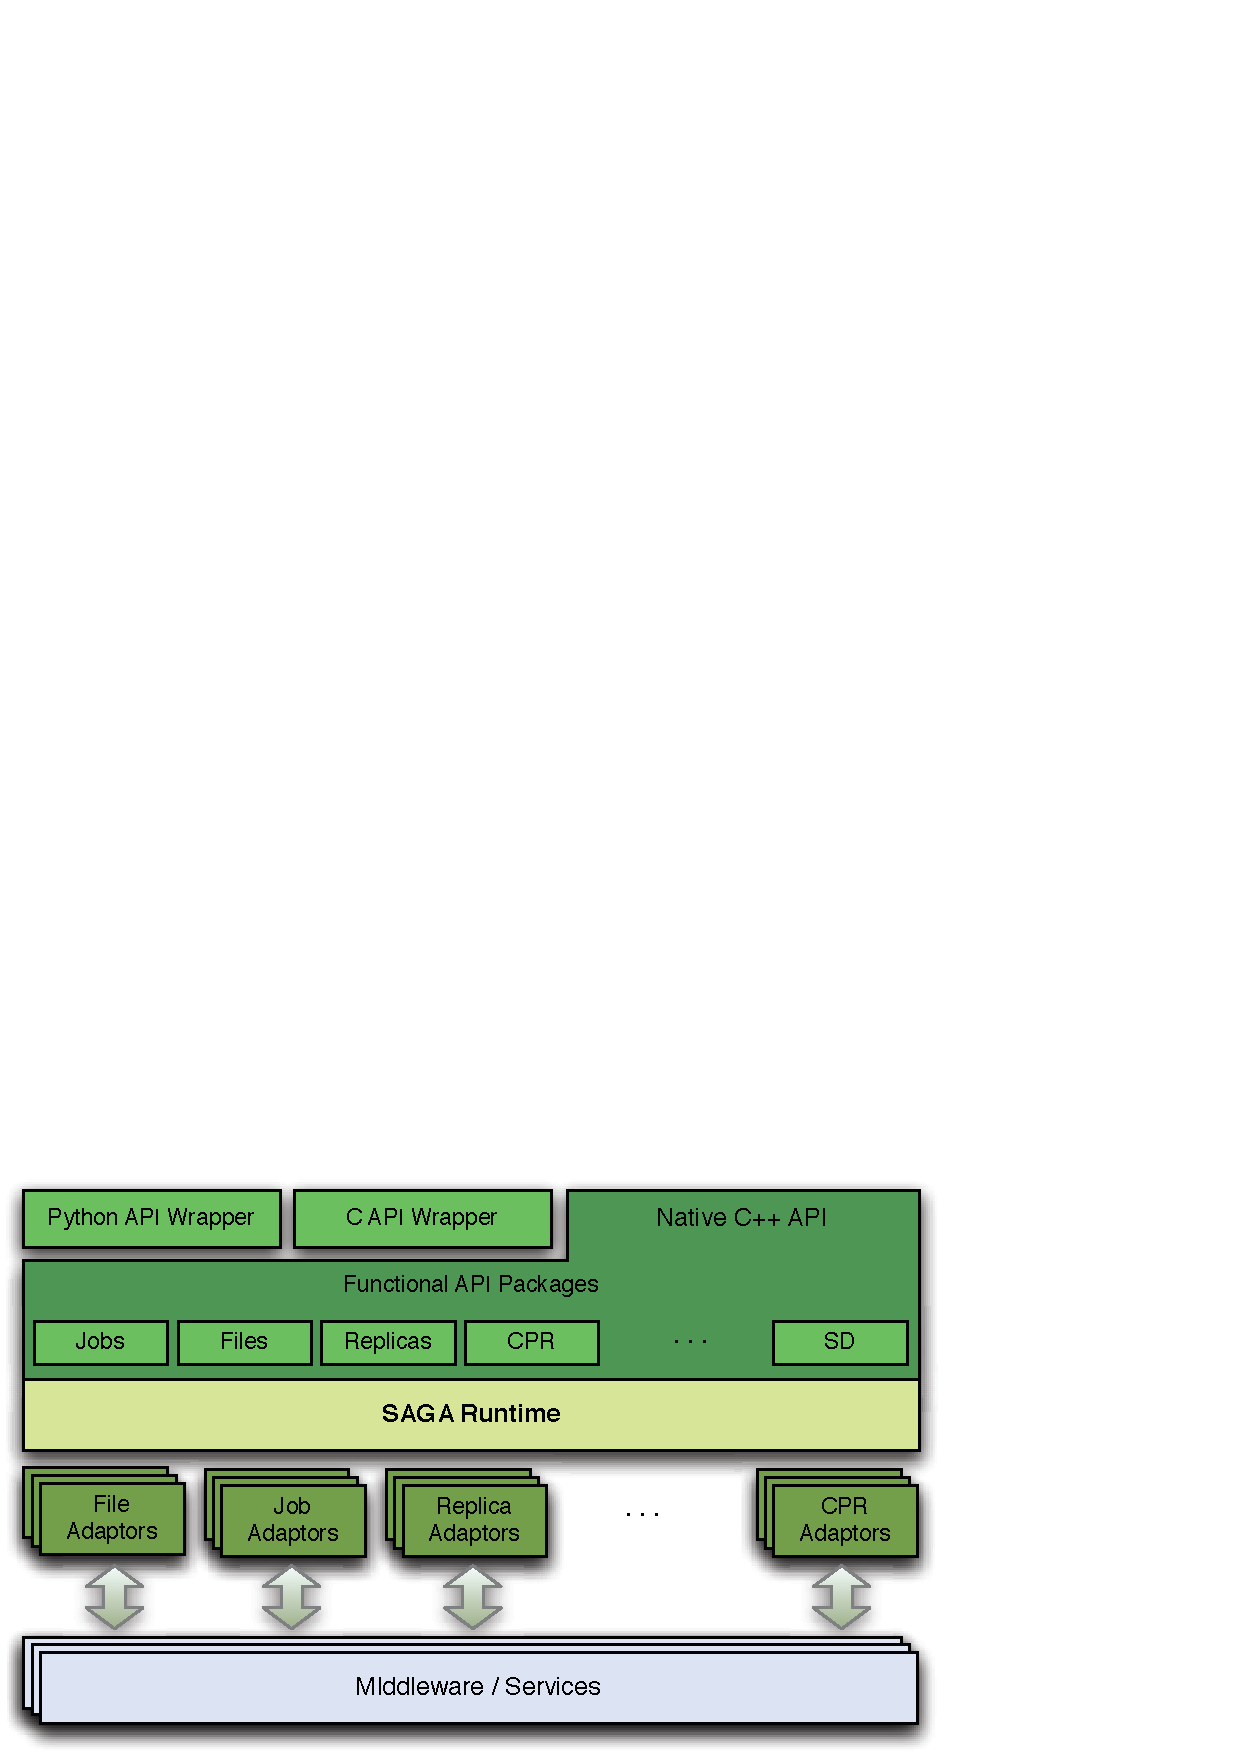
\includegraphics[scale=0.5]{saga-figure02.pdf}
\caption{In addition to the programmer's interface,
  the other important components of the landscape are the SAGA engine,
  and functional adaptors.} \vspace{-2em}
\label{saga_figure}
\end{figure}

Fig.~\ref{saga_figure} provide a view of the SAGA landscape, and the
main functional areas that SAGA provides a standardized interface
to. Based upon an analysis of more than twenty applications, the most
commonly required functionality involve job submission across
different distributed platforms, support for file access and transfer,
as well as logical file support. Less common, but equally critical,
wherever they were required, is the support for Checkpoint and
Recovery (CPR) and Service Discovery (SD).  The API is written in C++
with Python, C and Java language support. The {\it engine} is the main
library, which provides dynamic support for run-time environment
decision making through loading relevant adaptors. We will not discuss
details of SAGA here; details can be found elsewhere~\cite{saga_url}.

\section{Interfacing SAGA to Grids and Clouds}

\subsection{SAGA: An interface to Clouds and Grids}{\bf AM}

As mentioned in the previous section SAGA was originally developed for
Grids and that too mostly for compute intensive application. This was
as much a design decision as it was user-driven, i.e., the majority of
applications that motivated the design and formulation of version 1.0
of the API were HPC applications attempting to utilize distributed
resources.  Ref~\cite{saga_ccgrid09} demonstrated that in spite of its
original design constraints, SAGA can be used to control
data-intensive applications in diverse distributed environments,
including Clouds.  This in part is due to the fact that the
``distributed functionality'' required remains the same -- namely the
ability to submit jobs to different back-ends, the ability to move
files between distributed resources etc. Admittedly, and as we will
discuss, the semantics of, say the basic {\texttt job\_submit()}
changes in going from Grid enviroments to Cloud environments, but the
application remains oblivious of these changes and does not need to be
refactored. Specifically, {\texttt job\_submit()} when used in a Cloud
context results in the creation of a virtual machine instance and the
assignment of a job to that virtual machine; on the other hand, in the
context of Grids, {\texttt job\_submit()} results in the creation of a
job via a service and submission to GRAM style gatekeeper. In the
former the virtual machine is assigned to the saga::job and ...  In a
nutshell, this is the power of a high-level interface such as SAGA and
upon which the capability of interoperability is based.

\subsection{The Role of Adaptors} {\textcolor{blue} {AM}}

So how in spite of the significant change of the semantics does SAGA
keep the application immune to change? The basic feature that enables
this is a context-aware adaptor that is dynamically loaded....
\jhanote{The aim of the remainder of this section is to discuss how
  SAGA on Clouds differs from SAGA for Grids with specifics Everything
  from i) job submission ii) file transfer...iii) others..}


\subsection{Clouds Adaptors: Design and Implementation}



\begin{figure}[!ht]
\upp
 \begin{center}
  \begin{mycode}[label=SAGA Job Launch via GRAM gatekeeper]
   { // contact a GRAM gatekeeper
    saga::job::service     js;
    saga::job::description jd;
    jd.set_attribute (``Executable'', ``/tmp/my_prog'');
    // translate job description to RSL
    // submit RSL to gatekeeper, and obtain job handle
    saga:job::job j = js.create_job (jd);
    j.run ():
    // watch handle until job is finished
    j.wait ();
   } // break contact to GRAM
  \end{mycode}
  \caption{\label{gramjob}Job launch via Gram }
 \end{center}
\upp
\end{figure}

\begin{figure}[!ht]
\upp
 \begin{center}
  \begin{mycode}[label=SAGA create a VM instance on a Cloud]
   {// create a VM instance on Eucalyptus/Nimbus/EC2
    saga::job::service     js;
    saga::job::description jd;
    jd.set_attribute (``Executable'', ``/tmp/my_prog'');
    // translate job description to ssh command
    // run the ssh command on the VM
    saga:job::job j = js.create_job (jd);
    j.run ():
    // watch command until done
    j.wait ();
   } // shut down VM instance
  \end{mycode}
  \caption{\label{vmjob} Job launch via VM}
 \end{center}
\upp
\end{figure}

%{\bf SAGA-MapReduce on Clouds and Grids:} 
\begin{figure}[t]
  % \includegraphics[width=0.4\textwidth]{MapReduce_local_executiontime.png}
  \caption{Plots showing how the \tc for different data-set sizes
    varies with the number of workers employed.  For example, with
    larger data-set sizes although $t_{pp}$ increases, as the number
    of workers increases the workload per worker decreases, thus
    leading to an overall reduction in $T_c$. The advantages of a
    greater number of workers is manifest for larger data-sets.}
\label{grids1}
\end{figure}

% {\bf SAGA-MapReduce on Cloud-like infrastructure: } Accounting for the
% fact that time for chunking is not included, Yahoo's MapReduce takes a
% factor of 2 less time than \sagamapreduce
% (Fig.~\ref{mapreduce_timing_FS}). This is not surprising, as
% \sagamapreduce implementations have not been optimized, e.g.,
% \sagamapreduce is not multi-threaded.
% \begin{figure}[t]
% \upp
%       \centering
% %          \includegraphics[width=0.40\textwidth]{mapreduce_timing_FS.pdf}
%           \caption{\tc for \sagamapreduce using one worker (local to
%             the master) for different configurations.  The label
%             ``Hadoop'' represents Yahoo's MapReduce implementation;
%             \tc for Hadoop is without chunking, which takes
%             several hundred sec for larger data-sets.  The ``SAGA
%             MapReduce + Local FS'' corresponds to the use of the local
%             FS on Linux clusters, while the label ``SAGA + HDFS''
%             corresponds to the use of HDFS on the clusters. Due to
%             simplicity, of the Local FS, its performance beats
%             distributed FS when used in local mode.}
%           % It is interesting to note that as the data-set sizes get
%           % larger, HDFS starts outperforming local FS.  We attribute
%           % this to the use of caching and other advanced features in
%           % HDFS which prove to be useful, even though it is not being
%           % used in a distributed fashion.  scenarios considered are
%           % (i) all infrastructure is local and thus SAGA's local
%           % adapters are invoked, (ii) local job adaptors are used,
%           % but the hadoop file-system (HDFS) is used, (iii) Yahoo's
%           % mapreduce.
% %      \label{saga_mapreduce_1worker.png}
%           \label{mapreduce_timing_FS}
% \upp
% \end{figure}
% Experiment 5 (Table~\ref{exp4and5}) provides insight into performance
% figure when the same number of workers are available, but are either
% all localized, or are split evenly between two similar but distributed
% machines. It shows that to get lowest $T_c$, it is often required to
% both distribute the compute and lower the workload per worker; just
% lowering the workload per worker is not good enough as there is still
% a point of serialization (usually local I/O).  % It shows that when
% % workload per worker gets to a certain point, it is beneficial to
% % distribute the workers, as the machine I/0 becomes the bottleneck.
% When coupled with the advantages of a distributed FS, the ability to
% both distribute compute and data provides additional performance
% advantage, as shown by the values of $T_c$ for both distributed
% compute and DFS cases in Table~\ref{exp4and5}.

\section{SAGA-based MapReduce}

In this paper we will demonstrate the use of SAGA in implementing well
known programming patterns for data intensive computing.
Specifically, we have implemented MapReduce; we have also developed
real scientific applications using SAGA based implementations of these
patterns: multiple sequence alignment can be orchestrated using the
SAGA-All-pairs implementation, and genome searching can be implemented
using SAGA-MapReduce.

{\bf MapReduce:} MapReduce~\cite{mapreduce-paper} is a programming
framework which supports applications which operate on very large data
sets on clusters of computers.  MapReduce relies on a number of
capabilities of the underlying system, most related to file
operations.  Others are related to process/data
allocation. % The Google File-System, and other
% distributed file-systems (DFS), provide the relevant capabilities,
% such as atomic file renames.  Implementations of MapReduce on these
% DFS are free to focus on implementing the data-flow pipeline, which is
% the algorithmic core of the MapReduce framework.  
One feature worth noting in MapReduce is that the ultimate dataset is
not on one machine, it is partitioned on multiple machines distributed
over a Grid. Google uses their distributed file system (Google File
System) to keep track of where each file is located.  Additionally,
they coordinate this effort with Bigtable.

{\bf SAGA-MapReduce Implementation:} We have recently implemented
MapReduce in SAGA, where the system capabilities required by MapReduce
are usually not natively supported. Our implementation interleaves the
core logic with explicit instructions on where processes are to be
scheduled.  The advantage of this approach is that our implementation
is no longer bound to run on a system providing the appropriate
semantics originally required by MapReduce, and is portable to a
broader range of generic systems as well.  The drawback is that our
implementation is relatively more complex -- it needs to add system
semantic capabilities at some level, and it is inherently slower -- as
it is difficult to reproduce system-specific optimizations to work
generically.
% it is for these capabilities very difficult or near impossible to
% obtain system level performance on application level. 
Critically however, none of these complexities are transferred to the
end-user, and they remain hidden within the framework. Also many of
these are due to the early-stages of SAGA and incomplete
implementation of features, and not a fundamental limitation of the
design or concept of the interface or programming models that it
supports.

The overall architecture of the SAGA-MapReduce implementation is shown
in Fig.~\ref{saga-mapreduce_controlflow}. This simple interface
provides the complete functionality needed by any MapReduce algorithm,
while hiding the more complex functionality, such as chunking of the
input, sorting of the intermediate results, launching and coordinating
the map and reduce workers, etc. as implemented by the framework.  The
application consists of two independent processes, a master and worker
processes. The master process is responsible for:

\begin{figure}[t]
\centering
\includegraphics[width=0.4\textwidth]{saga-mapreduce_controlflow.png}
\caption{High-level control flow diagram for SAGA-MapReduce. SAGA uses
  a master-worker paradigm to implement the MapReduce pattern. The
  diagram shows that there are several different infrastructure
  options to a SAGA based
  application; % in particular for MapReduce there
  \jhanote{I think there should be something between the Map(1) and
    the Reduce(2) phases.. something that comes back to the Master,
    non?} \jhanote{We need to provide an arrow parallel to GRAM and
    Condor saying something like AWS or Eucalyptus}} \vspace{-2em}
      \label{saga-mapreduce_controlflow}
\end{figure}

\begin{itemize}
\item Launching all workers for the map and reduce steps as described
  in a configuration file provided by the user 
\item Coordinating the executed workers, including the chunking of the
  data, assigning the input data to the workers of the map step,
  handling the intermediate data files produced by the map step and
  passing the names of the sorted output files to the workers of the
  reduce step, and collecting the generated outputs from the reduce
  steps and relaunching single worker instances in case of failures,
\end{itemize}

The master process is readily available to the user and needs no
modification for different Map and Reduce functions to execute.  The
worker processes get assigned work either from the map or the reduce
step. The functionality for the different steps have to be provided by
the user, which means the user has to write 2 C++ functions
implementing the required MapReduce algorithm.
Fig.\ref{src:saga-mapreduce} shows a very simple example of a
MapReduce application to count the word frequencies in the input data
set. The user provided functions |map| (line 14) and |reduce| (line
25) are invoked by the MapReduce framework during the map and reduce
steps. The framework provides the URL of the input data chunk file to
the |map| function, which should call the function |emitIntermediate|
for each of the generated output key/value pairs (here the word and
it's count, i.e. '1', line 19). During the reduce step, after the data
has been sorted, this output data is passed to the |reduce|
function. The framework passes the key and a list of all data items
which have been associated with this key during the map step. The
reduce step calls the |emit| function (line 34) for each of the final
output elements (here: the word and its overall count). All key/value
pairs that are passed to |emit| will be combined by the framework into
a single output file.

As shown in Fig.~\ref{saga-mapreduce_controlflow} both, the master and
the worker processes use the SAGA-API as an abstract interface to the
used infrastructure, making the application portable between different
architectures and systems. The worker processes are launched using the
SAGA job package, allowing to launch the jobs either locally, using
Globus/GRAM, Amazon Web Services, or on a Condor pool. The
communication between the master and the worker processes is ensured
by using the SAGA advert package, abstracting an information database
in a platform independent way (this can also be achieved through
SAGA-Bigtable adaptors).  The Master process creates partitions of
data (referred to as chunking, analogous to Google's MapReduce), so
the data-set does not have to be on one machine and can be
distributed; this is an important mechanism to avoid limitations in
network bandwidth and data distribution.  These files could then be
recognized by a distributed File-System (FS) such as Hadoop-FS
(HDFS). All file transfer operations are based on the SAGA file
package, which supports a range of different FS and transfer
protocols, such as local-FS, Globus/GridFTP, KFS, and HDFS.


\section{SAGA-MapReduce on Clouds and Grids}

... Thanks to the low overhead of developing adaptors, SAGA has been
deployed on three Cloud Systems -- Amazon, Nimbus~\cite{nimbus} and
Eucalyptus~\cite{eucalyptus} (we have a local installation of
Eucalyptus, referred to as GumboCloud).  In this paper, we focus on
EC2 and Eucalyptus.


\subsection*{Infrastructure Used} We first describe the infrastructure
that we employ for the interoperabilty tests.

{\it Amazon EC2:}

{\it Eucalyptus, ECP:}

{\it Eucalyptus, GumboCloud:}

And describe LONI in a few sentences.  {\textcolor{blue}{KS}}


\subsection{Deployment Details}

We have also deployed \sagamapreduce to work on Cloud platforms.  It
is critical to mention that the \sagamapreduce code did not undergo
any changes whatsoever. The change lies in the run-time system and
deployment architecture. For example, when running \sagamapreduce on
EC2, the master process resides on one VM, while workers reside on
different VMs.  Depending on the available adaptors, Master and Worker
can either perform local I/O on a global/distributed file system, or
remote I/O on a remote, non-shared file systems.  In our current
implementation, the VMs hosting the master and workers share the same
ssh credentials and a shared file-system (using sshfs/FUSE).
Application deployment and configuration (as discussed above) are also
performed via that sshfs.  \jhanote{Andre, Kate please add on the
  above..}

On EC2, we created custom virtual machine (VM) image with
pre-installed SAGA.  For Eucalyptus, a boot strapping script equips a
standard VM instance with SAGA, and SAGA's prerequisites (mainly
boost).  To us, a mixed approach seemed most favourable, where the
bulk software installation is statically done via a custom VM image,
but software configuration and application deployment are done
dynamically during VM startup.  \jhanote{more details on how we create
  VMs, how we launch jobs and transfer files to these backend}

\subsection{Demonstrating Cloud-Grid Interoperabilty}

There are several aspects to Cloud Interoperability. A simple form of
interoperability -- more akin to inter-changeable -- is that any
application can use either of the three Clouds systems without any
changes to the application: the application simply needs to
instantiate a different set of security credentials for the respective
runtime environment, aka cloud.  Interestingly, SAGA provides this
level of interoperability quite trivially thanks to the adaptors.  By
almost trivial extension, SAGA also provides Grid-Cloud
interoperability, as shown in Fig.~\ref{gramjob} and ~\ref{vmjob},
where exactly the same interface and functional calls lead to job
submission on Grids or on Clouds. Although syntactically identical,
the semantics of the calls and back-end management are somewhat
different.  For example, for Grids, a \texttt{job\_service} instance
represents a live job submission endpoint, whilst for Clouds it
represents a VM instance created on the fly. 

\subsection{Experiments} In an earlier paper
(Ref~\cite{saga_ccgrid09}), we had carried out the following tests, to
demonstrate how \sagamapreduce utilizes different infrastructrure and
control over task-data placement, and gain insight into performance on
``vanilla'' Grids. Some specific tests we performed and used to
understand performance of \sagamapreduce in distributed environments
were:
\begin{enumerate}
\item We began by distributing \sagamapreduce workers (compute) and
  the data they operate on locally. We varied the number of workers
  vary from 1 to 10, and the data-set sizes varying from 1 to
  10GB. 
\item We then understood the effect of performance when using a
  distributed FS, that is we had \sagamapreduce workers compute local
  (to master), but using a distributed FS (HDFS). We varied
  the underlying distributed-FS (used KFS in lieu of HDFS).
% \item Same as Exp. \#2, but using a different distributed FS
%   (KFS); the number of workers varies from 1-10
% \item We then distributed the \sagamapreduce workers distributed compute (workers) and distributed file-system (KFS)
% \item Distributed compute (workers) but using local file-systems (using GridFTP for transfer)
\end{enumerate}

Mirroring the same strucuture, in this paper, we perform the following
experiments:
\begin{enumerate}
\item We take \sagamapreduce and compare its performance for the
  following configurations when exclusively running in Clouds to the
  performance in Grids: We vary the number of workers vary from 1 to
  10, and the data-set sizes varying from 1 to 10GB.  In these first
  set of experiments, we set the number of workers per VM to be 1,
  which is treated as the base case.  We perform these tests on both
  EC2 and using Eucalyptus.
\item For Clouds, we then vary the number of workers per VM, such that
  the ratio is 1:2; we repeat with the ratio at 1:4 -- that is the
  number of workers per VM is 4.
\item We then distribute the same number of workers across two
  different Clouds - EC2 and Eucalyptus.
\item Finally, for a single master, we distribute workers across Grids
  (LONI) and Clouds (EC2, with one job per VM). We compare the
  performance from the two hybrid (EC2-Grid, EC2-Eucalyptus
  distribution) cases to the pure distributed case.
% \item Distributed compute (workers) but using GridFTP for
%   transfer. This corresponds to the case where workers are able to
%   communicate directly with each other.  \jhanote{I doubt we will get
%     to this scenario, hence if we can do the above three, that is more
%     than enough.}
\end{enumerate}

It is worth reiterating, that although we have captured concrete
performance figures, it is not the aim of this work to analyze the
data and understand performance implications. It is the sole aim of
this work, to establish via well-structured and designed experiments
as outlined above, the fact that \sagamapreduce has been used to
demonstrate Cloud-Cloud interoperabilty and Cloud-Grid
interoperabilty.  The analysis of the data and understanding
performance involves the generation of ``system probles'', as there
are differences in the specific Cloud system implementation and
deployment. For example, in EC2 Clouds the default scenario is that
the VMs are distributed with respect to each other. There is notion of
availability zone, which is really just a control on which
data-center/cluster the VM is placed. In the absence of explicit
mention of the availabilty zone, it is difficult to determine or
assume that the availability zone is the same. However, for ECP and
GumboCloud, it can be established that the same cluster is used and
thus it is fair to assume that the VMs are local with respect to each
other.  Similarly, for data.. it should also be assumed that for
Eucalpytus based Clouds, data is also locally distributed (with
respect to a VM), whereas for EC2 clouds this cannot be assumed to be
true for every experiment/test. \jhanote{Andre, Kate please confirm
  that you agree with the last statment}

\subsubsection{Results}

Our image size is ... \jhanote{fix and provide details}

It takes SAGA about 45 seconds to instantiate a VM on Eucalyptus
\jhanote{Andre is this still true?}  and about 100 seconds on average
on EC2.  We find that the size of the image (say 5GB versus 20GB)
influences the time to instantiate an image EC2 somewhat, but is a
within instance-to-instance fluctuation.

Once instantiated, it takes about 1 second to assign a job to a VM on
Eucalyptus, or EC2.  It is a configurable option to tie the VM
lifetime to the \texttt{job\_service} object lifetime, or not.  It is
also a matter of simple configuration to determine how many jobs (in
this case workers) are assigned to a single VM. The default case is 1
worker per VM, but it is important to be able to vary the number of
workers per VM (just like in the Grid case we were able to vary the
number of workers per machine). 

% Due to space limitations we will not discuss the
% performance data of \sagamapreduce with different data-set sizes and
% varying worker numbers.

\subsubsection{Performance} The total time to completion ($T_c$) of a
\sagamapreduce job, can be decomposed into three primary components:
$t_{pp}$ defined as the time for pre-processing -- which in this case
is the time to chunk into fixed size data units, and to possibly
distribute them. This is in some ways the overhead of the process.
Another component of the overhead is the time it takes to instantiate
a VM. It is worth mentioning that currently we instantiate VMs
serially as opposed to doing this concurrently. This is not a design
decision but just a quirk, with a trivial fix to eliminate it.  Our
performance figures take the net instantiation time into account and
thus normalize for multiple VM instantiation -- whether serial or
concurrent. In other words, we will report figures where specific
start-up times have been removed and thus numbers indicate relative
performance and are amenable to direct comparision.  $t_{comp}$ is the
time to actually compute the map and reduce function on a given
worker, whilst $t_{coord}$ is the time taken to assign the payload to
a worker, update records and to possibly move workers to a destination
resource. $t_{coord}$ is indicative of the time that it takes to
assign chunks to workers and scales as the number of workers
increases. In general:

\vspace{-1em}
\begin{eqnarray}
T_c = t_{pp} + t_{comp} + t_{coord}
\end{eqnarray}


% \subsubsection{}

\begin{table}
\upp
\begin{tabular}{ccccc}
  \hline
  \multicolumn{2}{c}{Number-of-Workers}  &  data size   &  $T_c$  & $T_{spawn}$ \\   
  TeraGrid &  AWS &   (GB)  & (sec) & (sec)  \\
  \hline
  6 & 0 & 10   &  153.5 & 103  \\
  10 & 0 & 10  &  433.0  & 299 \\
  2 & 2 & 10 & 54.76 & 35.0 \\
  4 & 4 &10 & 188.0 & 135 \\
  10 & 10 & 10 & 1037.5 & 830 \\
  \hline
  0 & 10 & 100 &  845.0 & 632.0 \\
  1 & 1 & 100 & 29.04 & 9.79 \\
  \hline \hline
\end{tabular}
\upp
\caption{} 
\label{stuff}
\upp
\upp
\end{table}

\section{Discussion}

\subsection*{Related Programming Approaches}

We have chosen SAGA to implement MapReduce and control the distributed
features. However, in principle there are other approaches that could
have been used to control the distributed nature of the MapReduce
workers.

Some alternate approaches to using MapReduce could have employed
Sawzall and Pig~\cite{pig}.

Mention Sawzall~\cite{sawzall} as a language that builds upon
MapReduce; once could build Sawzall using SAGA.

Pig is a platform for large data sets that consists of a high-level
language for expressing data analysis programs, coupled with
infrastructure for evaluating these programs. The salient property of
Pig programs is that their structure is amenable to substantial
parallelization, which in turns enables them to handle very large data
sets.

Quick comparision of our approach with other approaches, including
those involving Google's BigEngine.


\subsubsection*{Challenges: Network, System Configuration and
  Experiment Details}

All this is new technology, hence makes sense to try to list some of
the challenges we faced. We need to outline the interesting Cloud
related challenges we encountered.  Not the low-level SAGA problems,
but all issues related to making SAGA work on Clouds.
{\textcolor{blue} Kate and Andre}

\subsubsection*{Programming Models for Clouds}

\jhanote{Mention that Amazon and Eucalyptus although distinct are
  somewhat similar; a very different beast is Google's AppEngine.  We
  will in the near future be working towards providing \sagamapreduce
  via Google's AppEngine}

  Programming Models Discuss affinity: Current Clouds
  compute-data affinity


%Simplicity of Cloud interface:

To a first approximation, interface determines the programming models
that can be supported. Thus there is the classical trade-off between
simplicity and completeness.  It is important to note that, some of
the programming models that are common to both data-intensive
application and Cloud-based computing, where there is an explicit
cost-model for data-movement, is to develop general heuristics on how
we handle common considerations such as when to move the data to the
machine or when to process it locally.

Complexity versus Completeness: There exist both technical reasons and
social engineering problems responsible for low uptake of Grids. One
universally accepted reason is the complexity of Grid systems -- the
interface, software stack and underlying complexity of deploying
distributed application. But this is also a consequence of the fact
that Grid interfaces tend to be ``complete'' or very close thereof.
For example, while certainly not true of all cases, consider the
following numbers, which we believe represent the above points well:
the Globus Toolkit Version 4.2 provides, in its Java version,
approximately 2,000 distinct method calls.  The complete SAGA Core
API~\cite{saga_gfd90} provides roughly 200 distinct method calls.  The
SOAP rendering of the Amazon EC2 cloud interface provides,
approximately 30 method calls (and similar for other Amazon Cloud
interfaces, such as Eucalyptus~\cite{eucalyptus_url}).  The number of
calls provided by these interfaces is no guarantee of simplicity of
use, but is a strong indicator of the extent of system semantics
exposed.

\section{Conclusion}

We have demonstrated the power of SAGA as a programming interface and
as a mechanism for codifying computational patterns, such as
MapReduce.  We have shown the power of abstractions for data-intensive
computing by demonstrating how SAGA, whilst providing the required
controls and supporting relevant programming models, can decouple the
development of applications from the deployment and details of the
run-time environment.

We have shown in this work how SAGA can be used to implement mapreduce
which then can utilize a wide range of underlying infrastructure. This
is one where how Grids will meet Clouds, though by now means the only
way. What is critical about this approach is that the application
remains insulated from any underlying changes in the infrastructure.

Patterns capture a dominant and recurring computational mode; by
providing explicit support for such patterns, end-users and domain
scientists can reformulate their scientific problems/applications so
as to use these patterns.  This provides further motivation for
abstractions at multiple-levels.

\section{Acknowledgments}

SJ acknowledges UK EPSRC grant number GR/D0766171/1 for supporting
SAGA and the e-Science Institute, Edinburgh for the research theme,
``Distributed Programming Abstractions''.  This work would not have
been possible without the efforts and support of other members of the
SAGA team.  In particular, \sagamapreduce was written by Chris and
Michael Miceli with assistance from Hartmut Kaiser; we also thank
Hartmut for great support during the testing and deployment phases of
this project. We are greatful to Dmitrii Zagorodnov (UCSB) and Archit
Kulshrestha (CyD group, CCT) for the support in deployment with
Eucalyptus.  We also acknowledge internal resources of the Center for
Computation \& Technology (CCT) at LSU and computer resources provided
by LONI.  \bibliographystyle{plain} \bibliography{saga_data_intensive}
\end{document}

\jhanote{We begin with the observation that the efficiency of
  \sagamapreduce is pretty close to 1, actually better than 1 -- like
  any good (data) parallel applications should be.  For 1GB data-set,
  \tc = 659s and for 10GB \tc = 6286s.  The efficiency remains at or
  around 1, even when the compute is distributed over two machines: 1
  worker at each site: \tc = 672s, \tc = 1081s and \tc =2051s for 1, 2
  and 4GB respectively; this trend is valid even when the number of
  workers per site is more than 1.

  Fig.~\ref{grids1} plots the \tc for different number of active
  workers on different data-set sizes; the plots can be understood
  using the framework provided by Equation 1. For each data-set (from
  1GB to 10GB) there is an overhead associated with chunking the data
  into 64MB pieces; the time required for this scales with the number
  of chunks created.  Thus for a fixed chunk-size (as is the case with
  our set-up), $t_{pp}$ scales with the data-set size. As the number
  of workers increases, the payload per worker decreases and this
  contributes to a decrease in time taken, but this is accompanied by
  a concomitant increase in $t_{coord}$. However, we will establish
  that the increase in $t_{coord}$ is less than the decrease in
  $t_{comp}$. Thus the curved decrease in \tc can be explained by a
  speedup due to lower payload as the number of workers increases
  whilst at the same time the $t_{coord}$ increases; although the
  former is linear, due to increasing value of the latter, the effect
  is a curve. The plateau value is dominated by $t_{pp}$ -- the
  overhead of chunking etc, and so increasing the number of workers
  beyond a point does not lead to a further reduction in \tc.

  To take a real example, we consider two data-sets, of sizes 1GB and
  5GB and vary the chunk size, between 32MB to the maximum size
  possible, i.e., chunk sizes of 1GB and 5GB respectively. In the
  configuration where there is only one chunk, $t_{pp}$ should be
  effectively zero (more likely a constant), and \tc will be dominated
  by the other two components -- $t_{comp}$ and $t_{coord}$.  For 1GB
  and 5GB, the ratio of \tc for this boundary case is very close to
  1:5, providing strong evidence that the $t_{comp}$ has the bulk
  contribution, as we expect $t_{coord}$ to remain mostly the same, as
  it scales either with the number of chunks and/or with the number of
  workers -- which icos the same in this case.  Even if $t_{coord}$
  does change, we do not expect it to scale by a factor of 5, while we
  do expect $t_{comp}$ to do so.

% Here we will by necessity
% limit our discussion to two type of distributed file-systems (HDFS and
% KFS) and two types of distributed structured-data store (Bigtable and
% HBase). We have developed SAGA adaptors for these, have used
% \sagamapreduce (and All-Pairs) seamlessly on these infrastructure.

% {\it HDFS and KFS: } HDFS is a distributed parallel fault tolerant
% application that handles the details of spreading data across multiple
% machines in a traditional hierarchical file organization.  Implemented
% in Java, HDFS is designed to run on commodity hardware while providing
% scalability and optimizations for large files.  The FS works by having
% one or two namenodes (masters) and many rack-aware datanodes (slaves).
% All data requests go through the namenode that uses block operations
% on each data node to properly assemble the data for the requesting
% application.  The goal of replication and rack-awareness is to improve
% reliability and data retrieval time based on locality.  In data
% intensive applications, these qualities are essential. KFS (also
% called CloudStore) is an open-source high-performance distributed FS
% implemented in C++, with many of the same design features as HDFS.

% There exist many other implementations of both distributed FS (such as
% Sector) and of distributed data-store (such as Cassandra and
% Hybertable); for the most part they are variants on the same theme
% technically, but with different language and performance criteria
% optimizations.  Hypertable is an open-source implementation of
% Bigtable; Cassandra is a Bigtable clone but eschews an explicit
% coordinator (Bigtable's Chubby, HBase's HMaster, Hypertable's
% Hyperspace) for a P2P/DHT approach for data distribution and location
% and for availability.  In the near future we will be providing
% adaptors for Sector\footnote{http://sector.sourceforge.net/} and
% Cassandra\footnote{http://code.google.com/p/the-cassandra-project/}.
% And although Fig.~\ref{saga_figure} explicitly maps out different
% functional areas for which SAGA adaptors exist, there can be multiple
% adaptors (for different systems) that implement that functionality;
% the SAGA run-time dynamically loads the correct adaptor, thus
% providing both an effective abstraction layer as well as an
% interesting means of providing interoperability between different
% Cloud-like infrastructure.  As testimony to the power of SAGA, the
% ability to create the relevant adaptors in a lightweight fashion and
% thus extend applications to different systems with minimal overhead is
% an important design feature and a significant requirement so as to be
% an effective programming abstraction layer.
